\PassOptionsToPackage{pdfpagelabels=false}{hyperref} 

\documentclass{beamer}

\usepackage[T1]{fontenc}
\usepackage[utf8]{inputenc}
\usepackage{lmodern}
%\usepackage[pdftex]{graphics}

\usepackage{graphicx}
\graphicspath{{img/}}
\DeclareGraphicsExtensions{.pdf,.png}

%\usetheme{Boadilla}
%\usetheme{Goettingen}
%\usetheme{Szeged}
\usetheme{total}
%\usecolortheme{Goettingen}

\title[NUMA aware framework]{\huge{NUMA aware framework for reservoir simulation}}
\author[Corentin Rossignon]{{\bf C. Rossignon}, P. H{é}non, O. Aumage and S. Thibault}
\institute[Total, Inria]{Total S.A., Inria Bordeaux, LaBRI, Universit{é} Bordeaux I}

\AtBeginSection[]
{
  \begin{frame}<beamer>
    \frametitle{Outline}
    \tableofcontents[currentsection]
  \end{frame}
}

\defbeamertemplate*{title page}{customized}[1][]
{
\begin{center}
  \usebeamercolor[fg]{titlelike}
  \usebeamerfont*{frametitle}
  \inserttitle\par
\end{center}
  
\begin{center}
  \usebeamerfont{subtitle}\insertsubtitle\par
  \bigskip
  \usebeamerfont{author}\insertauthor\par
  \usebeamerfont{institute}\insertinstitute\par
  \bigskip
  \usebeamerfont{date}\insertdate
  \bigskip
   
  \includegraphics[width=0.20\paperwidth]{TOTAL_SA}%
   \hspace*{0.05\paperwidth}~%
  \includegraphics[width=0.20\paperwidth]{inria}%
   \hspace*{0.05\paperwidth}~%
  
\includegraphics[width=0.10\paperwidth]{labri}%
   \hspace*{0.05\paperwidth}~%
  
\includegraphics[width=0.10\paperwidth]{bordeaux_1}
\end{center}
}

\usepackage{amsmath}
\begin{document}

\begin{frame}
  \titlepage
\end{frame}


\begin{frame}
  \frametitle{Outline}
  \tableofcontents
\end{frame}



%=========================================================
\section{Context}
%=========================================================
%-------------------------------
\begin{frame}
  \frametitle{What do we need for reservoir simulation ?}
  \centerline{\includegraphics[width=0.6\paperwidth]{reservoir}}

  \begin{itemize}
    \item Simulation over a period of decades :
    \begin{itemize}
      \item multi-day time steps
      \item must resolve several sparse linear systems
      \item septadiagonal matrices with millions of non-zeros
    \end{itemize}
    \item Use of preconditioned FGMRES
  \end{itemize}
\end{frame}

%-------------------------------
\begin{frame}
  \frametitle{Hierarchical architectures}
  \centerline{\includegraphics[width=0.9\linewidth]{numa_architecture}}

  \begin{itemize}
    \item NUMA\footnote{Non Uniform Memory Access} effect concerns most modern clusters
    \item Need two levels of parallelism :
      \begin{itemize}
        \item MPI : parallelism over nodes (domain decomposition)
        \item Thread : parallelism inside nodes (task based solution)
      \end{itemize}
  \end{itemize}
\end{frame}


%-------------------------------
\begin{frame}
  \frametitle{Task scheduling}
  
  \begin{block}{Task parallelism}
    A paradigm to parallelize code under a DAG\footnote{Direct Acyclic Graph} form
    where nodes are computation task and edges are dependencies between nodes.
  \end{block}

  \begin{itemize}
    \item Good paradigm for problems with data dependencies
    \item Programmer must define an appropriate grain size
  \end{itemize}
\end{frame}



%=========================================================
\section{Problems}
%=========================================================

%-------------------------------
\begin{frame}
  \frametitle{Problems of ILU(k)\footnote{Incomplete LU, mathematical method} factorization}
  
  Natural description of task parallelism, but:
  \begin{itemize}
   	\item Over 1 million tasks
   	\item 1 task duration is around $100\,ns$
   	\item 1 task management is approximately $500\,ns$
  \end{itemize}
  
  \begin{alertblock}{Problem 1}
    The grain size is too small.
  \end{alertblock}
  
  \begin{alertblock}{Problem 2}
    How to take advantage of machine topology ?
  \end{alertblock}
\end{frame}


%-------------------------------
%% \begin{frame}
%%   \frametitle{Example of DAG for an ILU(k) factorization}
  
%%   %   (-_-)   %
%%   \begin{figure}[t!]
%%     \centering
%%     \includegraphics[width=\linewidth]{G1}
%%     \caption{Very small case, a regular cube of 10 cells per side.}
%%   \end{figure}
  
%% \end{frame}

%=========================================================
\section{Task Coarsening}
%=========================================================
\begin{frame}
  \frametitle{Task coarsening}

  \centerline{\includegraphics[width=0.80\linewidth]{insert}}

  \begin{itemize}
    \item New step between the task description and DAG execution
    \item Involves increasing grain size by grouping tasks
  \end{itemize}
  
  \begin{block}{Task coarsening}
    From a finer DAG, we compute a coarser DAG by applying
    some generalist coarsening algorithms.
  \end{block}
\end{frame}


%-------------------------------
\begin{frame}
  \frametitle{Task coarsening - Algorithms}

  %   (-_-)   %
  \begin{figure}[t!]
    \centering
    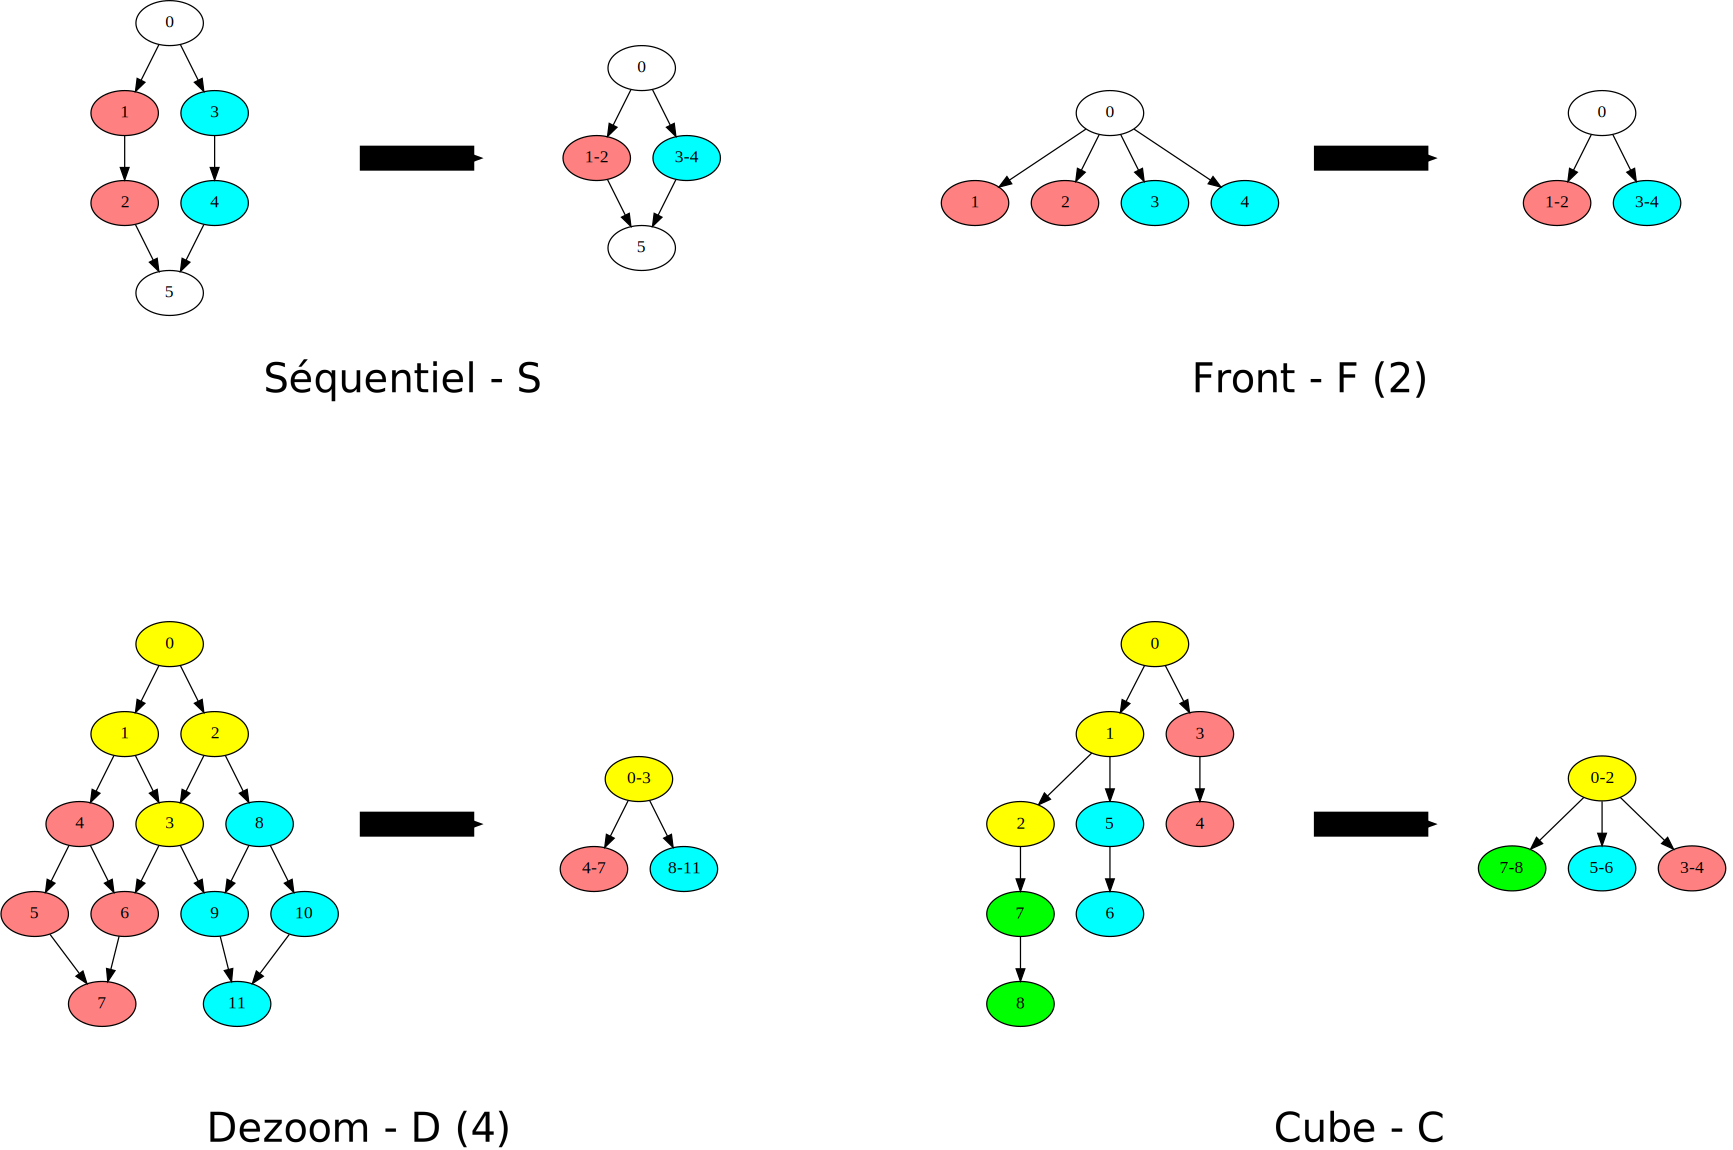
\includegraphics[width=\linewidth]{all_algo}
  \end{figure}
\end{frame}


%-------------------------------
\begin{frame}
  \frametitle{Example of task coarsening}

  %   (-_-)   %
  \begin{figure}[t!]
    \centering
    \includegraphics[width=0.7\linewidth]{G_agg}
    \caption{Aggregation CF(4) of a regular cube of 10 elements per side.}
  \end{figure}
\end{frame}


%-------------------------------
\begin{frame}[allowframebreaks]
  \frametitle{Example of coarsening with the Front algorithm}
  
  \centerline{\includegraphics[width=0.75\linewidth]{F4}}

  \begin{itemize}
    \item Width of DAG $\approx$ maximum number of tasks at same time
    \item Reduce width $\implies$ reduce contention in task scheduler
  \end{itemize}

\framebreak
    
  \centerline{\includegraphics[width=\linewidth]{F4_zoom}}
  \begin{itemize}
    \item For each level :
    \begin{itemize}
      \item limit group number
      \item similar group size
    \end{itemize}
    \item Useful when too many tasks compared to available CPUs
  \end{itemize}
\end{frame}

%-------------------------------
\begin{frame}
  \frametitle{Results}
  
  %   (-_-)   %
  \begin{figure}[t!]
    \centering
    \includegraphics[width=\linewidth]{agg_cube_100_spe10}
    \caption{Speed-up with and without CD(4)\footnote{Coarser string : Continuation Oriented + De-zoomed with parameter 4} aggregation.}
  \end{figure}
\end{frame}



%=========================================================
\section{NUMA distribution}
%=========================================================
\begin{frame}
  \frametitle{NUMA aware}

  \centerline{\includegraphics[width=0.8\linewidth]{numa_rb}}

  Requirement to use NUMA properly :
  \begin{itemize}
    \item Distribute tasks evenly over NUMA nodes
    \item Move memory pages close to the task execution core
  \end{itemize}
\end{frame}

%-------------------------------
\begin{frame}
  \frametitle{Nas - a NUMA Aware Scheduler}
  
  \begin{itemize}
    \item<1-> Currently, no NUMA aware scheduler exists
    \item<2-> We have written a very simple NUMA aware scheduler (Nas)
    \item<3-> Only one task queue per NUMA node
    \item<4-> Without NUMA effect, performance close to Intel TBB
  \end{itemize}
\end{frame}

%-------------------------------
\begin{frame}
  \frametitle{NUMA allocator}

  \centerline{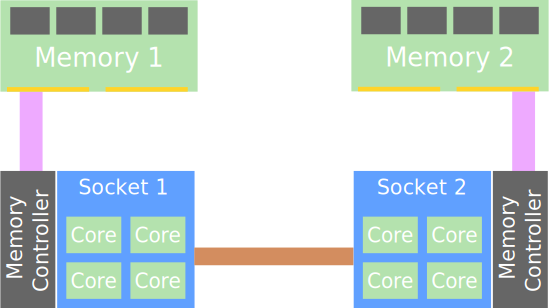
\includegraphics[width=\linewidth]{alloc_numa}}
  
  \begin{itemize}
    \item<1-> Linux default behavior is First Touch
    \item<2-> Interleaved allocation improves bandwidth
    \item<3-> Can be changed with ``numactl'' program
    \item<4-> NUMA allocators in Nas to match data locality with execution
    \item<5-> Beneficial effects on BLAS
  \end{itemize}
\end{frame}

%-------------------------------
\begin{frame}
  \frametitle{Results}
  
  %   (-_-)   %
  \begin{figure}[t!]
    \centering
    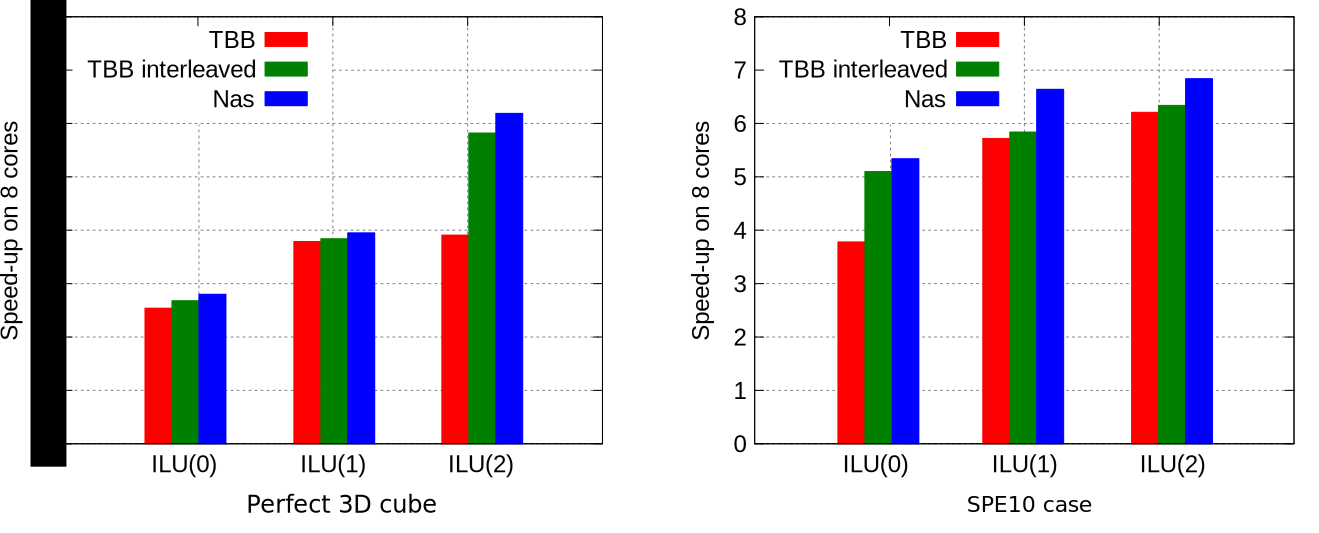
\includegraphics[width=\linewidth]{nas_cube_100_spe10}
    \caption{Speed-up comparing Intel TBB and our NUMA aware scheduler.}
  \end{figure}
\end{frame}

%=========================================================
\section{Conclusion and perspectives}
%=========================================================
%-------------------------------
\begin{frame}
  \frametitle{Conclusion and perspectives}
  	 Conclusion :
    \begin{itemize}
      \item<1-> Major improvement of the ILU(k) thanks to task aggregation
      \item<2-> The basic NUMA scheduler already increases performance
      \item<3-> Almost all BLAS can take advantage of NUMA allocator
    \end{itemize}
    \pause
    \pause
    \pause

 	 \bigskip
 	 \bigskip

    Perspectives :
    \begin{itemize}
      \item<4-> Improve NUMA integration with a cache-aware hierarchical scheduler
      \item<5-> Try aggregation on other problems
    \end{itemize}
\end{frame}

\section*{Questions}
%-------------------------------
\begin{frame}
  \frametitle{Thank you for your attention ...}
  
  \centerline{\includegraphics[width=0.25\linewidth]{questions}}
\end{frame}

\end{document}
